\documentclass[10pt, a4paper]{article}
\usepackage{lrec2006}
\usepackage{graphicx}

\usepackage[utf8]{inputenc}

\usepackage{alltt}  
\usepackage{tabularx}  
\usepackage{tipa}  

\usepackage{color}
\usepackage{relsize}
\usepackage{url}

\newcommand{\mytexttt}[1]{\texttt{\textscale{0.9}{#1}}}

\definecolor{MyGray}{rgb}{0.90,0.90,0.90}
\makeatletter\newenvironment{graybox}{%
   \begin{lrbox}{\@tempboxa}\begin{minipage}{.98\textwidth}}{\end{minipage}\end{lrbox}%
   \colorbox{MyGray}{\usebox{\@tempboxa}}
}\makeatother


\title{Dbnary: Wiktionary as a LMF based Multilingual RDF network}

\name{Gilles Sérasset}

\address{UJF-Grenoble 1, Laboratoire d'Informatique de Grenoble\\ 
GETALP Team, BP 53, 38051 Grenoble cedex 9, France \\ 
\texttt{gilles.serasset@imag.fr}
\\}


\abstract{Contributive resources, such as wikipedia, have proved to be valuable in Natural Language Processing or Multilingual Information Retrieval applications.
This article focusses on Wiktionary, the dictionary part of the collaborative resources sponsored by the \emph{Wikimedia} foundation.\\
In this article we present a word net that has been extracted from French, English and German wiktionaries. We present the structure of this word net and discuss the specific extraction problems induced by this kind of contributive resources and the method used to overcome them. \\
Then we show how we represent the extracted data as a Lexical Markup Framework (LMF) compatible lexical network represented in Resource Description Framework (RDF) format.\\
\textbf{Keywords:} Wiktionary, Multilingual Lexical Database, Lexical Networks, LMF, RDF.
}

\begin{document}

\maketitleabstract

\section{Introduction}

Wiktionary is a huge and free resource available on the web. Its main advantages are the presence of definitions that could help for disambiguation tasks and the large number of translations to many different languages. The drawback of this resource is the fact that the entries are described using a wiki syntax specifying the \emph{form} of the entry rather than its \emph{structure}. Moreover this description is sometime erroneous or heterogeneous.

The goal of the dbnary project is to provide an extraction process that produces a lexical word net as detailed as possible from wiktionary dumps. The extracted data can be used, as is, in another project\footnote{Latest extracted data is available at \mytexttt{http://kaiko.getalp.org/dbnary/}} or the extraction process itself can be integrated into another tool (for example, to have an on-demand extraction using the latest available data) as it is available as part of an open source project \footnote{\mytexttt{http://dbnary.forge.imag.fr/}}. Many efforts have already been attempted to use wiktionary data in NLP applications. Most of them were ad-hoc efforts and some of them provided either an API to, or an XML dump of, the extracted data. But the wiktionary data is an \emph{evolving} resource. It means that the data \emph{along with its encoding} changes while time goes on. Hence, the extraction program has to cope with the evolving usages of the contributors. Moreover, each wiktionary language edition uses its own encoding and usages to represent lexical information. We do believe that we can solve both problems by providing the extracted data \emph{and} the extraction program as an open source system.

In this paper, we will first give a very short and general description of the lexical structure of the main language editions of wiktionary. Then we address the main difficulties we met when extracting data from the different wiktionary dumps. We will then show how the extraction program is organized to allow its maintenance and extension by its users. Finally we will present the structure of the extracted data that is based on Lexical Markup Framework (LMF) standard, and stored as a RDF graph.

\section{Wiktionary and its data}

\subsection{Overview}

Wiktionary\footnote{\mytexttt{http://www.wiktionary.org/}} is a web based collaborative effort led by the Wikimedia foundation\footnote{\mytexttt{http://www.wikimedia.org/}} to build a free content dictionary in many languages.

\subsection{Macro- and Micro- Structures}

\cite{TUD-CS-2012-0008} give an extended description of wiktionary. In this section, we will provide an overview of the elements that are pertinent to this study.

Wiktionary organizes its data in a way that may be surprising for a lexicographer. This may be explained by the contributive approach used for building the resources and by the intended user experience. The key concepts used in wiktionary guidelines are also mainly motivated by the technology used to pursue this collaborative effort. 
% This section presents this organization by detailing its macro-structure (the way the articles are organized and/or related) and its micro-structure (the internal structure of each article).

Wiktionary is organized as a set of wiktionary \emph{language editions} (one per language) containing a set of \emph{pages} characterized by a \emph{page name}. Each page contains lexical data from different languages. In a wiktionary language edition (say the edition of language $l_1$), all lexical data (including data from other languages) are described using language $l_1$. 

Dictionary articles may be related to other articles in the same language edition (via lexico-semantic or translation links). They may also be related by translation links to articles on another edition. Pages may also be related to pages with the same \emph{page name} in other editions. 

Under this organization, each edition is (ultimately) intended to contain all lexical data of all languages described in the edition language.

\begin{figure*}[htb]
\begin{graybox}
\scriptsize
\begin{tabularx}{\textwidth}{llX}
\textbf{Page}&\emph{chat}&\\
\textbf{~Language*}& \texttt{1 English}&\textit{English language comes first in the English wiktionary}\\
&\texttt{1.1 Pronunciation}\footnote{\scriptsize This particular entry does not follow the rule that states that pronunciation should be given \emph{after} the Etymology.}\\
\textbf{~~~Etymology*}&\texttt{1.2 Etymology 1}& \textit{Etymology is used to distinguish homographs}\\
\textbf{~~~~~Core entry\footnote{\scriptsize This term is the one used in English Wiktionary guidelines.}}*&\texttt{1.2.1 Verb}& \textit{The core entry contains the definitions of the entry}\\
\textbf{~~~~~~~Definition}*&\emph{~~~To be engaged in informal conversation.}& \textit{list of word senses, described by their definitions, along with examples.}\\
&\texttt{\ldots}&\\
\textbf{~~~~~~~LexRels}*& & \textit{list of lexico-semantic relations}\\
\textbf{~~~~~~~Translation}*&\emph{~~~Danish: snakke, sludre}& \textit{list of translations grouped by word senses when available}\\
&\texttt{1.2.2 Noun}&\textit{Core entries are distinguished by their part of speech}\\
&\texttt{1.3 Etymology 2}\\
&\texttt{1.3.1 Noun}\\
&\texttt{3 Dutch}&\textit{Entries in other languages are structured according to the same principles}\\
&\texttt{4 French}
\\
&\texttt{\ldots}&\\
\end{tabularx}
\end{graybox}
\caption{Annotated table of contents of the entry ``chat'' in the English wiktionary.}\label{englishEntry}
\end{figure*}

\subsection{Anatomy of a wiktionary page}

While the details of the structure of lexical data differs between wiktionary language editions, wiktionary uses a common general abstract structure similar to the one found in main paper dictionaries. We illustrate this general structure with the structure of a page on the English server. Figure \ref{englishEntry} shows the annotated table of contents of \emph{``chat''} page on the English edition\footnote{This example has been extracted in february 2012. It is likely that the entry changed since then.}.

\begin{figure}[htb]
\resizebox{\linewidth}{!}{%
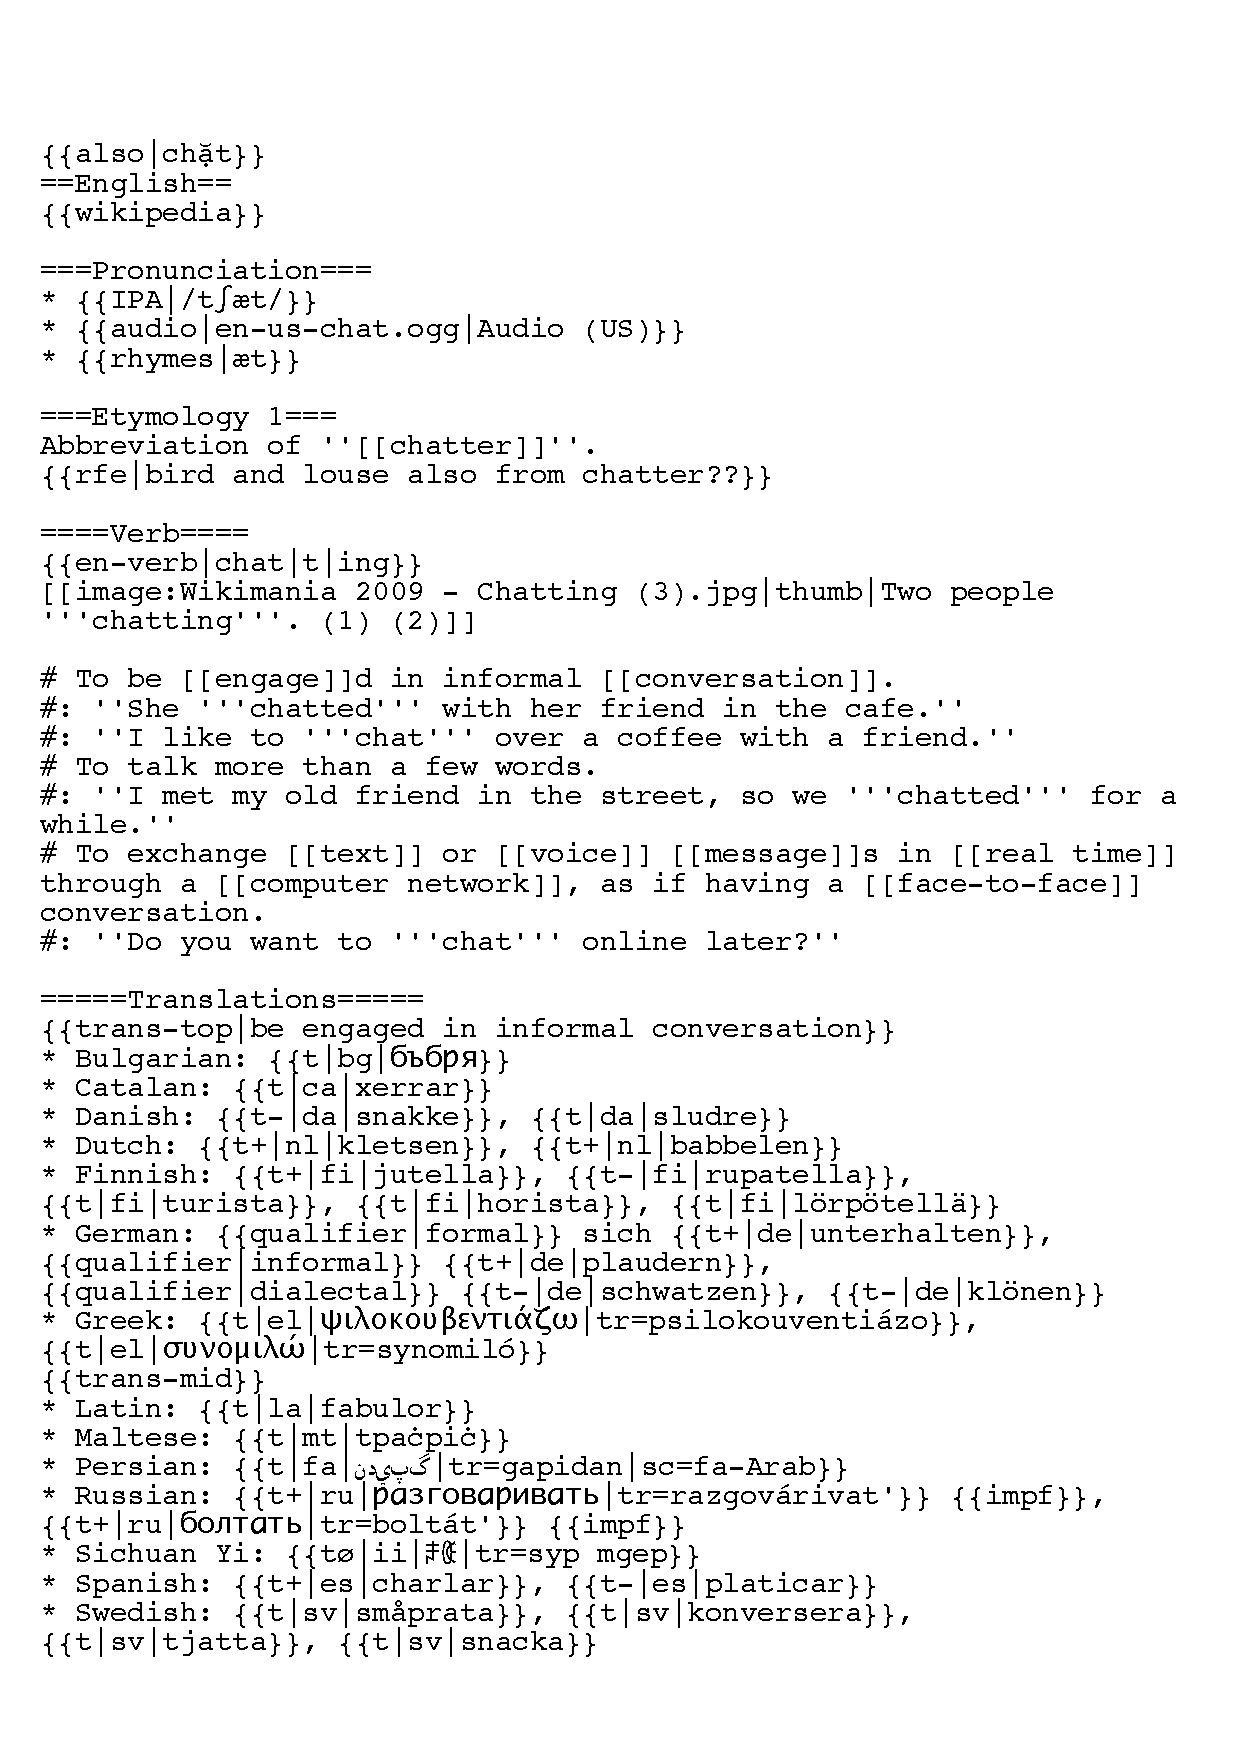
\includegraphics{chat1.pdf}
}
\caption{Excerpt of the entry ``chat'', as available in the English language edition, in mediawiki syntax.}
\label{extr:sample}
\end{figure}

\subsection{Internal representation of a wiktionary page}

All collaborative efforts led by the Wikimedia foundation involves the use of wikis to collect semi-structured collaborative data. The software used for these wikis is MediaWiki \cite{mediawiki.org}. Under MediaWiki, each page is defined using a specific syntax that describes its \emph{formatting}. This formatting language may be extended by defining \emph{templates} that will be expanded during page rendering. 
Most wiktionary language editions use specific templates to help users format their contributed lexical data in a coherent way. Figure \ref{extr:sample} shows a sample of the internal representation of the entry ``chat'', in the English language edition, where one can note some templates (surrounded by double curly braces) and links (surrounded by double square brackets). Figure \ref{extr:samplefr} gives an excerpt of the entry ``chat'' in the French language edition.

\begin{figure}[htb]
\resizebox{\linewidth}{!}{%
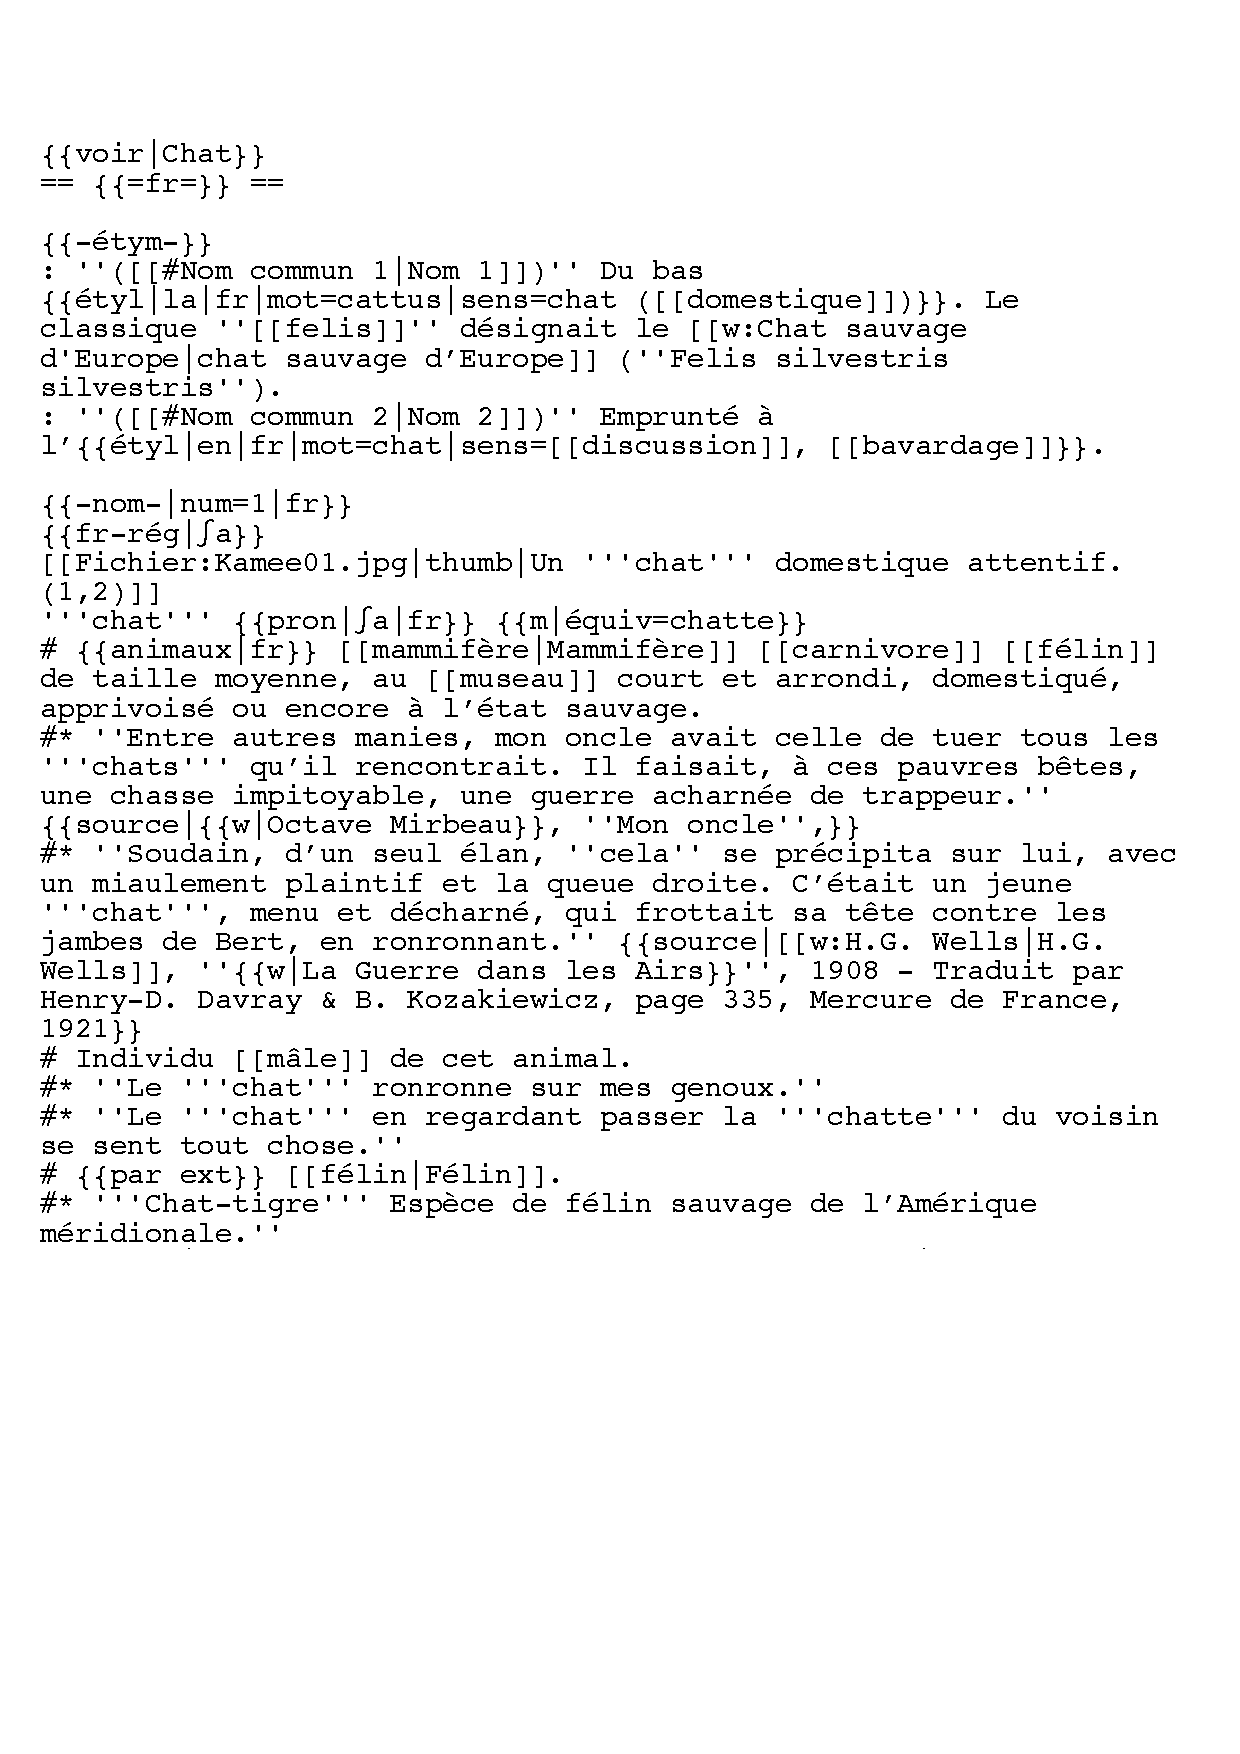
\includegraphics{chat2.pdf}
}
\caption{Excerpt of the entry ``chat'', as available in the French language edition, in mediawiki syntax.}
\label{extr:samplefr}
\end{figure}


The Wikimedia foundation provides a monthly dump\footnote{\mytexttt{http://dumps.wikimedia.org/}} of all pages of a wiktionary in this formatting language.

The dumps are extracted and encoded as UTF-16 text file. The extraction process goes through all pages in the dump file (using the provided xml based structure). Then each page is parsed using a finite state automaton implemented in java. The general abstract structure of entries is taken into account by a common abstract class while language specific details are refined through a language specific implementation class.

\section{Specific Problems and Extraction Process}

\subsection{Related work and motivation of our approach}

Many projects addressed wiktionary data extraction. For instance, \cite{sajous-EtAl-IceTAL2010} uses \emph{WiktionaryX}, an XML version of a 2010 wiktionary dump for French and English, available at \cite{WiktionaryX}. \cite{ZeschMuellerGurevych2008} provide a free to use, but closed-source, java library to programmatically access the data of the English and German wiktionaries. Other projects did use wiktionary based data in NLP applications without providing details on the way this data were extracted.

As stated in \cite{sajous-EtAl-IceTAL2010}, ``\emph{When merging information extracted from several languages, the homogenisation of the data structure often leads to the choice of the poorest one, resulting in a loss of information.}''. In this work we did not try to provide a uniform entry representation for all languages but rather used a simple lexical network model to represent as much data as we can extract correctly from the wiktionary dumps. We also chose to ignore some of the structure to ease the extraction process.

\begin{description}
\item[Lexical Entry] The wiktionary unit of information is a \emph{page}. While classical resources often create different lexical entries for homonyms, we chose to keep the wiktionary approach. Hence, each lexical entry in the extracted data corresponds to a unique page in wiktionary.
\item[Homonymy and Polysemy] If two words are homonyms, they will be described in the same page. In wiktionary the homonyms will be distinguished by different \emph{etymologies}. It is quite difficult to coherently extract homonyms (and gather word senses under the correct etymology) as entries in different language editions are very incoherent on this aspect. For instance, in the French edition, there should be only 1 etymology section (each etymology being numbered), and other part of speech sections will make reference to the corresponding etymology. On the other hand, in the English edition, several etymology sections will be used, each one preceding the part of speech (and word senses) it covers. Hence, we chose to ignore etymology and gather all word senses in a flat list in the lexical entry.
\item[Lexico Semantic Relations and translation links] For the very same reasons, it is most of the time not possible to reliably attach a lexicon semantic relation to its correct word sense. For instance, in the French entry ``chat'', ``matou'' is a synonym  of the word sense defined by ``chat mâle'' while ``minet'' is a synonym of the general word sense defined by ``chat domestique''. The same goes for translation links. We chose to attach such relations to the lexical entry rather than to its word senses, as the current attempts led to too many errors in the extracted data. However, whenever possible, we kept in the extracted structure the different \emph{hints}\footnote{e.g. many translations are grouped under an annotation that is usually a summary of a previous definition.} that are given in wiktionary. With such an approach we may be able to later re-attach the correct translations to the correct word senses by processing the extracted data, while a subset of entries may be processed with an ad-hoc extractor tailored to extract a gold standard for this task. 
\end{description}

All the above mentioned project do stress that the data is sometimes erroneous and most of the time heterogeneous. Among errors and incoherences one may find:

\begin{description}
\item [Unconventional encoding of structuring elements] For instance, in French, the main language section titles are encoded using a set of templates, named using the ISO 639-1 2 letters language codes \cite{ISO639-1:2002}. Here, \texttt{== \{\{=fr=\}\} ==} encodes the section heading ``Français''. Some French contributors did not use this templates but used \texttt{== Français ==} which leads to the very same rendering.
\item [Multiple templates may encode the same information] For instance, translation equivalents are gathered in boxes which are titled using a summary of a preceding definition. Such boxes represent a word sense for which the translations are valid. In the French language edition, such boxes may be created either with the \texttt{\{\{boîte début|...\}\}} template or with the \texttt{\{\{(|...\}\}} template. As both templates are quite common, the extraction process must recognize both of them.
\item [Syntactically incorrect elements] Some entries do contain templates that are syntactically ill-formed (e.g. a template is opened with curly braces and closed by square brackets).
\item [Order of the sections] Even when the templates are correctly used, the order of the different sections does not necessarily follows the recommendations available in the documentation. For instance, in the English wiktionary, contributors are asked to put pronunciation section after the etymology. In the entry ``chat'' that we gave as an example in Figure \ref{extr:sample}, this order is inverted. 
\end{description}

\subsection{Organization of the extractor}

As stated above, the errors and incoherence that are inherent to this contributive resource make things rather complicated for building of a generic extractor. Moreover, we want to use the many wiktionary language editions as a whole, interoperable, lexical network. Hence we need a tool that will be easy to adapt to a new language edition. 

We also want to keep the evolving nature of wiktionary, so that the available data will stay as synchronized as possible with the evolution of the resource. For this, we need to adapt the extractor to the evolving usages of the contributors that add new information but also change the templates themselves. This means that the extractor should be easy to change. This aspect is crucial in the context of a multilingual extractor.

For all these reasons, we focus on building an extractor that is:

\begin{itemize}
\item open-source: so that it is very easy to anyone to adapt it to his own needs,
\item based on LGPL license: so that we encourage users to provide their own tunings and heuristics to the main code base,
\item efficient: so that one may be able to do the extraction process on the fly, either from a dump, or directly from the online data, 
\item simple: we do not require any additional software installation as we do not use any database and we provide a simple build method based on \texttt{maven}\footnote{\url{http://maven.apache.org/}} that takes care of library dependencies.
\item with several tools: along with the extractor, we provide several development tools (e.g. a ``grep in wiktionary'' tool where you can find all wiktionary entries containing a certain pattern, or a ``get the raw entry'' of a page in the dump which may come handy when your dump file is around 4 Gb). 
\end{itemize}

The extractor itself is a java program containing 2 kind of classes:

\begin{itemize}
\item \texttt{WiktionaryExtractor} which parse the wiktionary entry and
\item \texttt{WiktionaryDataHandler} which store the extracted data
\end{itemize}

The Wiktionary extractor is an abstract class that handles general WikiMedia syntax (links, templates, etc.) and language independent processing. Language specific classes inherit from it and define the different \emph{patterns} that are used to structure the lexical entries in the language edition. This way the addition of a new language mainly consists in identifying regular expressions that match the different elements structuring the entry (section headers) and the different elements containing data to be extracted (translation templates, definition patterns, ...).

The \emph{WiktionaryExtractor} class and its children classes parse the entry and trigger methods of the \emph{WiktionaryDataHandler}. It is the responsibility of the data handler to structure and store the extracted data. This way, it is possible to adapt the extraction process to a new extracted data organization.

In this extraction process some heuristics are used to capture heterogeneous or erroneous data. But, as the wiktionary evolves (along with its conventions) and as the extraction program is adapted with new heuristics, one has to ensure that the extraction does not regress. For this, we use the Mulling tool provided by \cite{archer:2010} to compute the differences between extracted graphs. Such difference may be quickly evaluated and the extraction heuristics may be adopted or rejected accordingly.

\section{Extracted Data}

\subsection{Macro- and Micro- Structures}

Each language edition is extracted as a lexical network. This network is represented using the W3C standard \emph{Resource Description Framework} (RDF), as described in \cite{Klyne_Carroll_2004}. This structure is stored using the \emph{Turtle} textual syntax which is compact and easy to read \cite{Beckett06}, hence easing the debugging process. The English language network describes the English lexical entries (giving their part of speech, definitions, lexical relations and translations) while the French one describes the French lexical entries. Each lexical network is stored in a single Turtle file. 

The nodes and relations in this lexical network are typed using the classes defined in the Lexical Markup Framework (ISO/TC37/SC4) specification \cite{LMF-ISO,FRANCOPOULO:2006:INRIA-00121468:1}. LMF defines a set of classes using UML notation. These classes have been converted in RDF concepts under a specific name space (e.g. LMF \emph{Lexical Entry} class is described by the RDF \url{http://www.lexicalmarkupframework.org/lmf/r14\#LexicalEntry} resource).

Unlike the previous effort to create an RDF version of the LMF standard, we did not reified the relation between classes, but rather used simple RDF statements (properties) to avoid cluttering the extracted resource.

Every lexical network node is identified by an IRI, an internationalized URI that allows the use of non ASCII \emph{letters}, \cite{IRI-RFC3987}. For instance, the English lexical entry ``chat'' is identified by \url{http://getalp.org/dbnary/eng#chat} while the French lexical entry ``chat'' is identified by \url{http://getalp.org/dbnary/fra#chat}. 

The extracted network contains nodes from the LMF core package (\emph{Lexical Entry}, \emph{Sense}, \emph{Definition}), the LMF morphology package (\emph{Lemma}) the LMF Machine Readable Dictionary extension (\emph{Equivalent}). The standard is not strictly applied here, as one node named \emph{LexicalEntryRelation} has been introduced (an equivalent of the LMF Sense Relation class, but relating lexical entries rather than senses). Moreover, the \emph{Equivalent} relation relates a lexical entry rather than a sense as stated in the LMF standard.

A lexical entry node has a single \texttt{partOfSpeech} property. It may have several values, as the English entry ``chat'' which may be a verb and a noun. All sense nodes are related to their lexical entry by an \texttt{isPartOf} property. They also have a \texttt{partOfSpeech} property, which should have only one value. A definition is related to its corresponding sense by the \texttt{isPartOf} property. Lemmas are related to the lexical entry by an \texttt{isPartOf} property. A lemma is always created with the wiktionary page name as its \texttt{writtenForm} property. Additional lemmas are created when we detect alternative spellings in the wiktionary data.

Equivalence nodes are related to their corresponding lexical entry by an \texttt{isPartOf} property. They have a mandatory \texttt{language} property which value is the normalized ISO 639-3 3 letter language code \cite{ISO639-3:2007} of the translation. They also have a mandatory \texttt{writtenForm} property whose value is the written form of the translation. They may also have a \texttt{glose} property that contains the hint given in wiktionary to identify the sense for which the translation is valid. Finally, they may contain a \texttt{usage} property that contains some elements that are associated to individual translations. Its value depends on the language edition usages and the language of the translation. For instance, the French language edition sometimes give an indication on the usage or level of language. It also consistently gives the transliteration of all russian equivalents in Roman writing system.

Lexical entry relation nodes represent several types of relations:

\begin{itemize}
\addtolength{\itemsep}{-0.5\baselineskip}
%\item \texttt{def} relation which relates a lemma node with its definitions,
%\item \texttt{alt} relation which relates lemmas to their alternate spellings,
\item \texttt{ant} relation which relates lemmas to their antonyms,
\item \texttt{holo} relation which relates lemmas to their holonyms,
\item \texttt{hyper} relation which relates lemmas to their hypernyms,
\item \texttt{hypo} relation which relates lemmas to their hyponyms,
\item \texttt{mero} relation which relates lemmas to their meronyms,
\item \texttt{syn} relation which relates lemmas to their synonyms,
\item \texttt{qsyn} relation which relates lemmas to their quasi-synonyms (this one is only used in the French language edition),
%\item \texttt{trad} relation which related lemmas to their translation, this relation is annotated by the target language and by an optional glose that helps disambiguate the translated word sense.
\end{itemize}
 
Using this lexical network structure, we ignore many of the information available in wiktionaries, either because we do not want to use it in later processing or because it involves far more heuristics during data extraction.

%Figure \ref{chatWordNet} shows a sample of the extracted data in graphical format.

\subsection{Example of an extracted lexical entry}

Figure \ref{extr:chatrdfen} gives an excerpt of the lexical network for the English entry ``chat'' in Turtle format. Figure \ref{extr:chatrdfenuml} gives an UML like overview of the same excerpt.


\begin{figure}[htb]
\resizebox{\linewidth}{!}{%
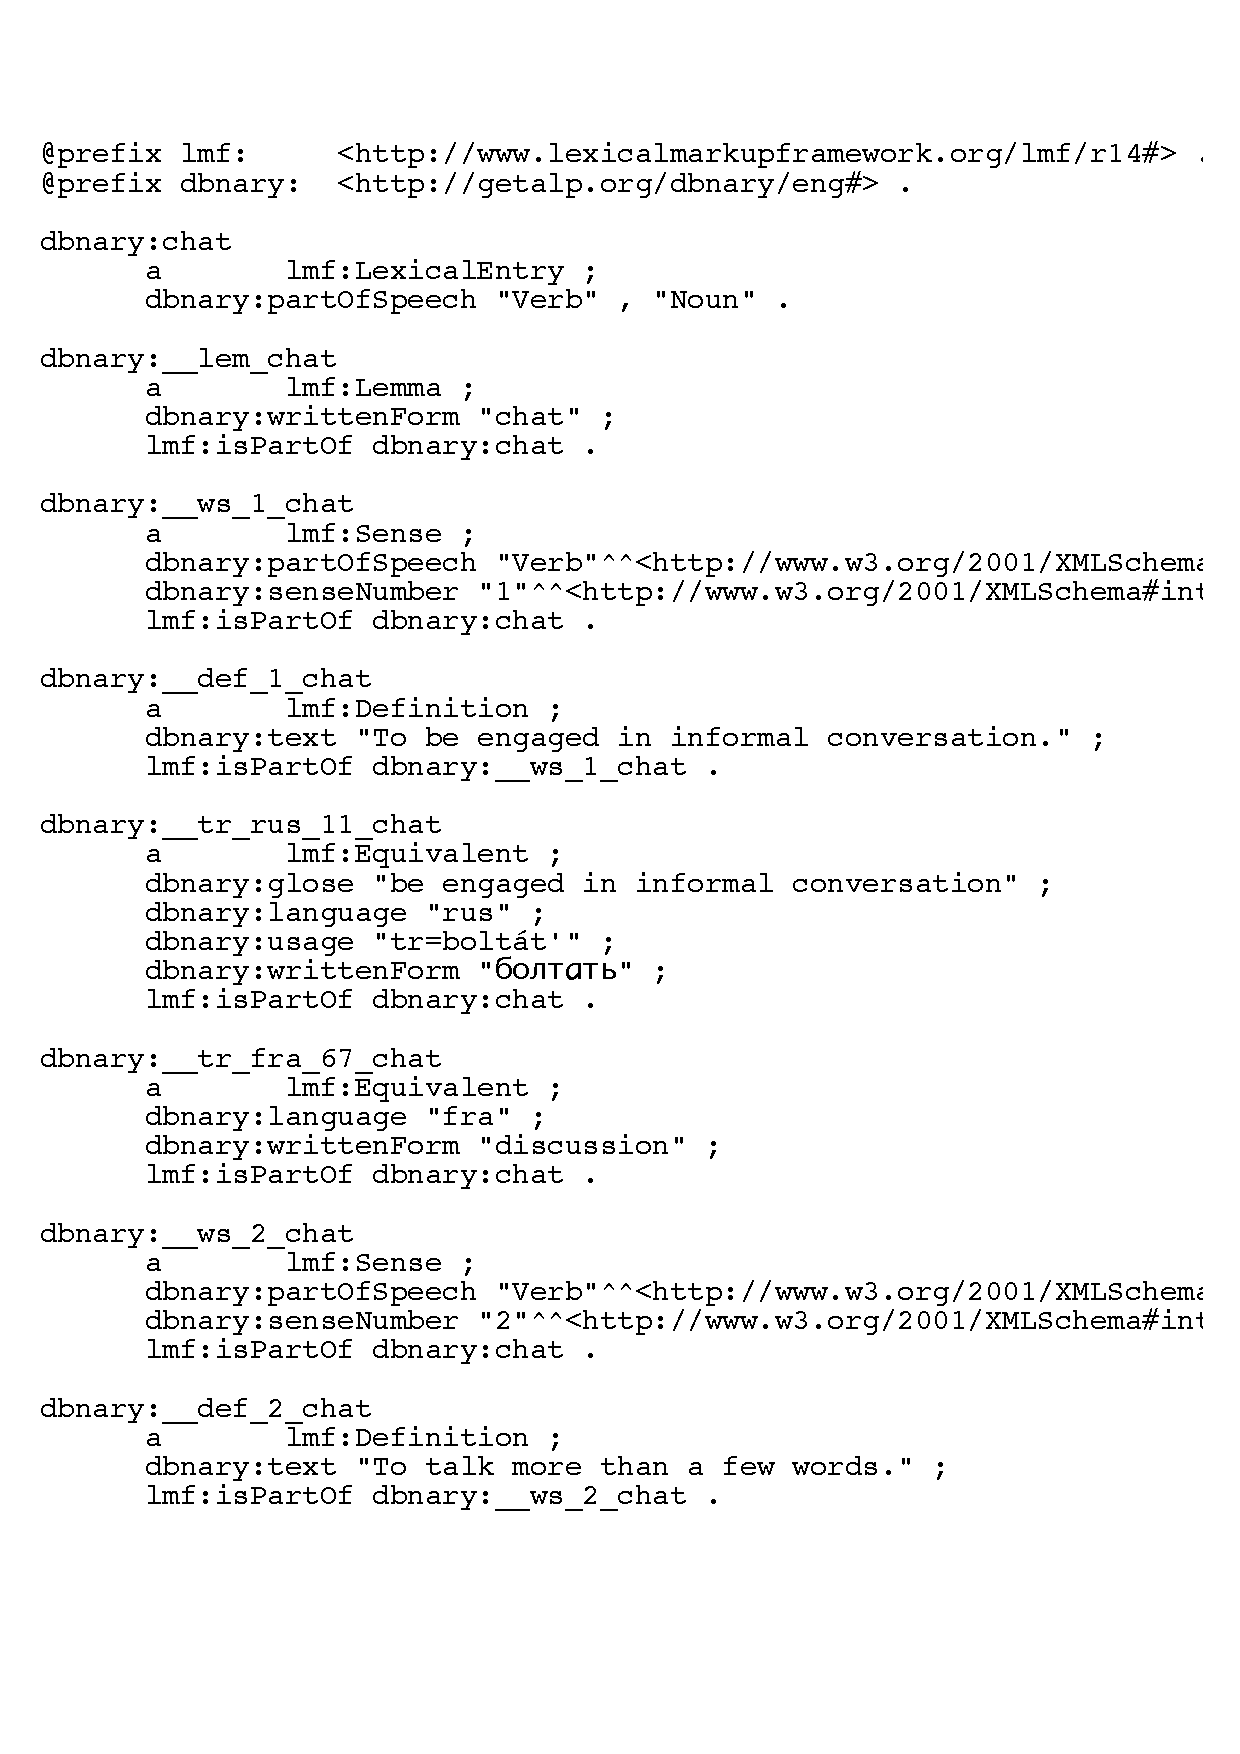
\includegraphics{chatrdfen.pdf}
}
\caption{Excerpt of the extracted network for the English entry ``chat'', in turtle syntax.}
\label{extr:chatrdfen}
\end{figure}

\begin{figure}[htb]
\resizebox{\linewidth}{!}{%
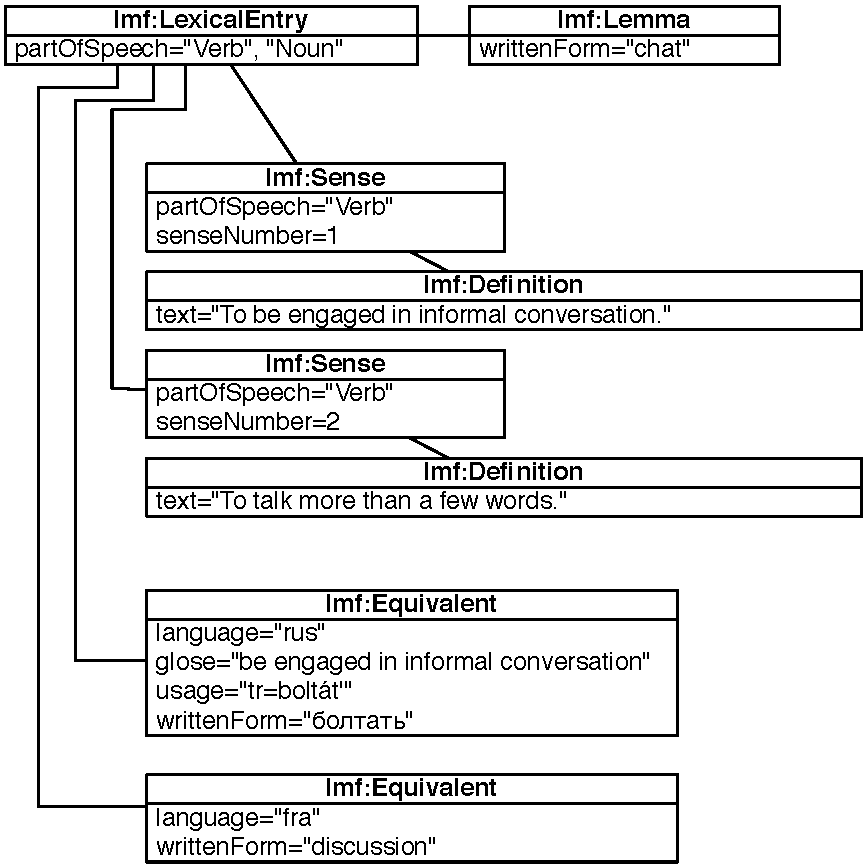
\includegraphics{chatrdfen-uml.pdf}
}
\caption{Excerpt of the extracted network for the English entry ``chat'', as an UML like network.}
\label{extr:chatrdfenuml}
\end{figure}


\subsection{Size of the involved data}

At the time of writing, we extracted data from the most up to date dump files of English ($4.1$ Gb), French ($3.1$ Gb) and German ($631$ Mb) wiktionaries. The full extraction of the English wiktionary takes around 4 min. on a 2.67 GHz Intel Xeon processor with enough memory to avoid swapping ($\sim 800$ Mb) as the lexical network is stored in memory during extraction.

% and Portuguese ($397$ Mb)

Table \ref{table:size} shows the size of the resulting networks.

%-rw-r--r--. 1 serasset geta 608M Oct 13 22:03 dewkt.xml
%-rw-r--r--. 1 serasset geta 3.9G Oct 13 22:02 enwkt.xml
%-rw-r--r--. 1 serasset geta 3.0G Oct 13 21:59 frwkt.xml
%-rw-r--r--. 1 serasset geta 390M Oct 13 22:03 ptwkt.xml

%Stats on RDF file: file:///Users/serasset/dev/wiktionary/extracts/RDF20120305/fr_extract_20120305.tut
%260467 lexical entries.
%246168 lemmas.
%395227 equivalents.
%106151 relations.
%330681 definitions.
%330681 senses.
%1669375 total nodes.
%ant: 8760
%holo: 5415
%hyper: 11272
%hypo: 17601
%mero: 4996
%qsyn: 2666
%syn: 55434
%fra translation in frawiktionary for entry[http://getalp.org/dbnary/fra#__tr_fra_4_crocodile_nain, http://www.lexicalmarkupframework.org/lmf/r14#isPartOf, http://getalp.org/dbnary/fra#crocodile_nain]
%source & eng & fra & deu  & others //
%fra & 73168 & 24 & 31589 & 290190//%394971
%
%
%Stats on RDF file: file:///Users/serasset/dev/wiktionary/extracts/RDF20120305/de_extract_20120305.tut
%155258 lexical entries.
%90207 lemmas.
%417687 equivalents.
%215085 relations.
%80934 definitions.
%80934 senses.
%1040105 total nodes.
%ant: 34691
%hyper: 49051
%hypo: 54733
%syn: 76606
%deu translation in deuwiktionary for entry[http://getalp.org/dbnary/deu#__tr_deu_5_Pantherpilz, http://www.lexicalmarkupframework.org/lmf/r14#isPartOf, http://getalp.org/dbnary/deu#Pantherpilz]
%source & eng & fra & deu  & others //
%deu & 68305 & 57400 & 4 & 291605//%417314
%
%
%Stats on RDF file: file:///Users/serasset/dev/wiktionary/extracts/RDF20120305/en_extract_20120305.tut
%414929 lexical entries.
%402442 lemmas.
%497204 equivalents.
%79487 relations.
%354359 definitions.
%354359 senses.
%2102780 total nodes.
%ant: 9964
%hyper: 1047
%hypo: 3144
%mero: 224
%syn: 65103
%eng translation in engwiktionary for entry[http://getalp.org/dbnary/eng#__tr_eng_1_obsolescence, http://www.lexicalmarkupframework.org/lmf/r14#isPartOf, http://getalp.org/dbnary/eng#obsolescence]
%source & eng & fra & deu  & others //
%eng & 0 & 33290 & 32083 & 430898//%496271


\begin{table}[htb]
\begin{minipage}{\linewidth}
\begin{tabular}{lrrr}
\multicolumn{4}{l}{\textbf{Nodes in graphs}}\\
\hline
			& English & French & German \\
entries &  414929 &  260467  &  155258  \\
lemmas 	& 402442  & 246168 & 90207  \\
definitions\footnote{The current English extraction program does not yet correctly recognize inflected forms. Hence, many lexical entries represent word forms and many of them are not related to a definition.}\footnote{There is exactly one definition node per sense node. Hence, sense node are not shown here, but they are counted in the total number of nodes.}
			& 354359 & 330681 & 80934 \\
relations  & 79487 & 106151 & 215085 \\
equivalents & 497204 & 395227 & 417687 \\
Total		& 2102780 & 1669375 & 1040105\\
\multicolumn{4}{l}{\textbf{Relations in graphs}}\\
\hline
syn	& 65103& 55434& 76606\\
qsyn\footnote{This relation is only available in French language edition. Other language editions do not distinguish between synonyms and quasi synonyms.}
	& -& 2666 & -\\
ant	& 9964& 8760& 34691\\
holo	& 0  & 5415& 0 \\
mero	& 224& 4996&0 \\
hyper	& 1047& 11272& 49051\\
hypo	& 3144& 17601& 54733\\
\end{tabular}
\end{minipage}
\caption{Size of the extracted lexical networks.}
\label{table:size}
\end{table}

%\begin{table*}[htb]
%\begin{minipage}{.9\linewidth}
%\begin{tabular}{lrrrr}
%\multicolumn{5}{l}{\textbf{Nodes in graphs}}\\
%\hline
%			& English & French & German \\
%lemmas 	& $372773$  & $ 236215 $ & $51111$  & $35979$\\
%definitions\footnote{The current English extraction script does not yet correctly recognize inflected forms. Hence, word nodes do not represent lemmas, but word forms and many word nodes are not related to a definition.}
%			& $321637$ & 283493 & 72539 & 57281\\
%other nodes\footnote{Other nodes are: lemmas that are not described in the wiktionary and lemmas or word forms in foreign languages}
%			& 320994 & 315610 & 333549 & 186565\\
%Total		& 1015404 & 835318 &457199 & 279825 \\
%\multicolumn{5}{l}{\textbf{Relations in graphs}}\\
%\hline
%syn	& 59102& 53548& 74641&13228\\
%qsyn	& 0& 2509 & 0&0\\
%ant	& 9092& 8494& 34158&1650\\
%holo	& 0  & 5491& 0 &0\\
%mero	& 198& 4949&0 &0\\
%hyper	& 906& 10438& 47785&2\\
%hypo	& 2718& 16571& 53175&10\\
%\end{tabular}
%\end{minipage}
%\caption{Size of the extracted lexical networks.}
%\label{extr:size}
%\end{table*}

As can be seen in table \ref{table:size} the number of relation is quite surprising in the German wiktionary. At the time of writing we do not have explanations on this figure and we still have to figure out if these relations are errors in the extraction process or problems in the wiktionary data itself. Errors are quite likely as the German wiktionary makes extensive use of nested macros which are difficult to correctly parse with our current automata based architecture.

Table \ref{table:translations} gives more details on the translation equivalents that have been extracted from the 3 wiktionary language editions. It lists the number of translation to the 17 largest language editions of wiktionaries, as found in the English, French and German language editions.

\begin{table*}[htb]
\begin{minipage}{.9\linewidth}
\begin{tabular}{lrrrrrrrrrrrr}
\textbf{from/to}  & deu & ell & eng & fin & fra & hun & ido & ita & lit & nor & pol & por \\
\textbf{deu} & 5 & 2362 & 68306 & 4429 & 57401 & 6874 & 340 & 33146 & 1663 & 4017 & 14918 & 8344 \\
\textbf{eng} & 32084 & 10718 & 1 & 48577 & 33291 & 13225 & 1496 & 27160 & 1899 & 7837 & 12156 & 15652\\
\textbf{fra} & 31590 & 6465 & 73169 & 6934 & 25\footnote{These are errors in the wiktionary data, where, for instance, the entry ``crocodile nain'' contains translations to Lingala that are tagged as French translations.} & 4926 & 11548 & 15310 & 1611 & 4129 & 7126 & 16735 \\
\hline
\textbf{from/to}  & rus & tam & tur & vie & zho& others & Total \\
\textbf{deu} & 19533 & 216 & 4192 & 426 & 7926 & 183589 & 234098\\
\textbf{eng} & 22314 & 165 & 6525 & 2250 & 51 & 261803 & 235401\\
\textbf{fra} & 6783 & 565 & 3667 & 1333 & 4030 & 199281 & 195946\\
\end{tabular}
\end{minipage}
\caption{Number of translation equivalent (for the considered languages) in the 17 largest wiktionary editions (sorted by alphabetical order on the 3 letters language code).}
\label{table:translations}
\end{table*}



%283493
%[serasset@brahms1 RAW_20111013]$ grep -c -- "-O- #def" en_extract.raw 
%321637
%[serasset@brahms1 RAW_20111013]$ grep -c -- "-O- #def" de_extract.raw 
%72539
%[serasset@brahms1 RAW_20111013]$ grep -c -- "-O- #def" pt_extract.raw 
%57281


%fr: 2176403 entries extracted in : 74163
%Semnet contains: 835318 nodes and 1372755 edges.
%
%de: 214984 entries extracted in : 90629
%Semnet contains: 457199 nodes and 742846 edges.
%
%en: 2803195 entries extracted in : 75379
%Semnet contains: 1015404 nodes and 1571179 edges.
%
%pt: 210889 entries extracted in : 13962
%Semnet contains: 279825 nodes and 386887 edges.
%
%[serasset@brahms2 RAW_20111013]$ grep -c -- "-O- #deu" de_extract.raw 
%51111
%[serasset@brahms2 RAW_20111013]$ grep -c -- "-O- #fra" fr_extract.raw 
%236215
%[serasset@brahms2 RAW_20111013]$ grep -c -- "-O- #eng" en_extract.raw 
%372773
%[serasset@brahms2 RAW_20111013]$ grep -c -- "-O- #por" pt_extract.raw 
%35979
%
%fr - alt : 39
%fr - ant : 8494
%fr - def : 323277
%fr - holo : 5491
%fr - hyper : 10438
%fr - hypo : 16571
%fr - mero : 4949
%fr - pos : 569820
%fr - qsyn : 2509
%fr - syn : 53548
%en - alt : 59
%en - ant : 9092
%en - def : 332743
%en - holo : 0
%en - hyper : 906
%en - hypo : 2718
%en - mero : 198
%en - pos : 732355
%en - qsyn : 0
%en - syn : 59102
%de - alt : 13
%de - ant : 34158
%de - def : 78849
%de - holo : 0
%de - hyper : 47785
%de - hypo : 53175
%de - mero : 0
%de - pos : 130875
%de - qsyn : 0
%de - syn : 74641
%pt - alt : 0
%pt - ant : 1650
%pt - def : 69547
%pt - holo : 0
%pt - hyper : 2
%pt - hypo : 10
%pt - mero : 0
%pt - pos : 107513
%pt - qsyn : 0
%pt - syn : 13228


%\subsection{Resulting lexical network}

\section{Conclusion}

The current paper shows preliminary results on an open source tool to extract a LMF based lexical network from different wiktionary language editions. Such a work is interesting for many users that will be able to use the extracted data in their own NLP system. Moreover, as the extracted resource uses the Resource Description Framework (RDF) standard and the Lexical Markup Framework (LMF) structure, the extracted data is also directly usable for researchers on the Semantic Web, where it could be used to ease the ontology alignment systems when terms in different languages are used to describe ontologies of a domain.

As the lexical network is formatted in RDF format, it is immediately usable by many existing tools (Ontology builders, Sparql query engines, reasoners...).

Our final objective is to create a tool that will be to wiktionary what dbpedia \cite{Auer07dbpedia:a} is to wikipedia. 

Our next objectives are to better generalize the treatments of the current extractors, so that it will be easier to create extractors for other languages. We are currently forking on Portuguese and we welcome all initiative aiming at the addition of new language to this open-source tool.

\section{Acknowledgements}

The work presented in this paper was conducted in the Videosense project, funded by the French National Research Agency (ANR) under its CONTINT 2009 programme (grant ANR-09-CORD-026).

\bibliographystyle{lrec2006}      % basic style, author-year citations
\bibliography{biblio}   % name your BibTeX data base

%\nocite{*}
\end{document}

